% \iffalse meta-comment
%
%% File: pdfresources.dtx
%
% Copyright (C) 2019 The LaTeX3 Project
%
% It may be distributed and/or modified under the conditions of the
% LaTeX Project Public License (LPPL), either version 1.3c of this
% license or (at your option) any later version.  The latest version
% of this license is in the file
%
%    https://www.latex-project.org/lppl.txt
%
% This file is part of the "pdfresources bundle" (The Work in LPPL)
% and all files in that bundle must be distributed together.
%
% -----------------------------------------------------------------------
%
% The development version of the bundle can be found at
%
%    https://github.com/latex3/latex3
%
% for those people who are interested.
%
%<*driver>
\documentclass{l3doc}
\PassOptionsToPackage{svgnames}{xcolor}
\usepackage{tabularx,array,booktabs}
\usepackage{AlegreyaSans}
\setmainfont{Heuristica}
\usepackage{tikzlings,csquotes,graphicx}
\usepackage[most]{tcolorbox}
\usetikzlibrary{patterns,patterns.meta}
\newcommand\bearwearlogo{{\sffamily\fontsize{10pt}{12pt}\selectfont
BearWear\raisebox{1ex}[0pt][0pt]{\textcircled{
\begin{tikzpicture}[baseline={(0,0.03)},scale=0.1]
\bear
\end{tikzpicture}}}}}
\newcommand{\TikZ}{Ti\emph{k}Z}
\lstdefinestyle{bearwarestyle}{% stolen and adapted from tikzlings
	language={[latex]TeX},
	tabsize=2,
	breaklines,
	basicstyle=\ttfamily,
	commentstyle={\color{green!50!black}\slshape},
	columns=fullflexible,
	alsodigit={-},
	alsoletter={3},
	emphstyle=\color{red!60!black},
	emph=[1]{
		tikzlings,
		tikzlings-marmots, tikzlings-bears, tikzlings-coatis, tikzlings-koalas, tikzlings-marmots, tikzlings-owls, tikzlings-penguins, tikzlings-snowmans, tikzlings-mice, tikzlings-moles, tikzlings-sloths, tikzlings-pigs, tikzlings-cats, tikzlings-hippos, tikzlings-rhinos, tikzlings-pandas,
		body, 3D, rotatehead, sideward, blush, sleeping, whiskers, teeth, shadow, askphil, leftstep, rightstep, eye, nose, pupil, bill, feet, belly, ask, phil, mouth, buttons, rotatearms, eyes, paws, back,
		scale, yshift, xshift, rotate, hands, muzzle, schroedinger, toes,
		hat, tophat, beret, strawhat, ribbon, harlequin, niuqelrah, witch, magichat, magicstars, crown, queencrown, kingcrown, santa, chef, graduate, tassel, alien, book, bookcolour, signpost, signcolour, signback, speech, think, bubblecolour, pizza, cheese, baguette, cake, icecream, flavoura, flavourb, flavourc, milkshake, wine, cricket, hockey, football, crystalball, magicwand, rollingpin, lightsaber, torch, basket, easter, egga, eggb, eggc, crozier, shovel, pickaxe, umbrella, umbrellaclosed, handbag, cocktail, pupilwidth,
	},
	texcsstyle=*\color{SteelBlue!50!black}\bfseries,
	keywordstyle=\color{red!60!black}\bfseries,
	morekeywords={tikzpicture},
	moretexcs={
		usepackage, usetikzlibrary, marmot, coati, bear, koala, owl, penguin, thing, tikzling, snowman, mouse, moles, sloth, pig, cat, hippo, rhino, panda,
	},
	delim ={[s][\ttfamily\color{green!50!black}]{$}{$}},
	moredelim=[is][\footnotesize\ttfamily\color{orange!70!black}]{|}{|},
	index=[1][emph]
}
\tcbset{%
	colframe=SteelBlue!50!black,
	arc=0mm,
	fonttitle=\bfseries,
	sidebyside,
	listing options={style=bearwarestyle},
	center lower,
	righthand width=6.5cm,
	bottom=0pt,
	top=0pt,
	tikz lower,
	height plus=3cm,
	colback=SteelBlue!30!white
}
\lstset{style=bearwarestyle}
\raggedbottom
\begin{document}
  \DocInput{\jobname.dtx}
\end{document}
%</driver>
% \fi
% \section{Interview}
% 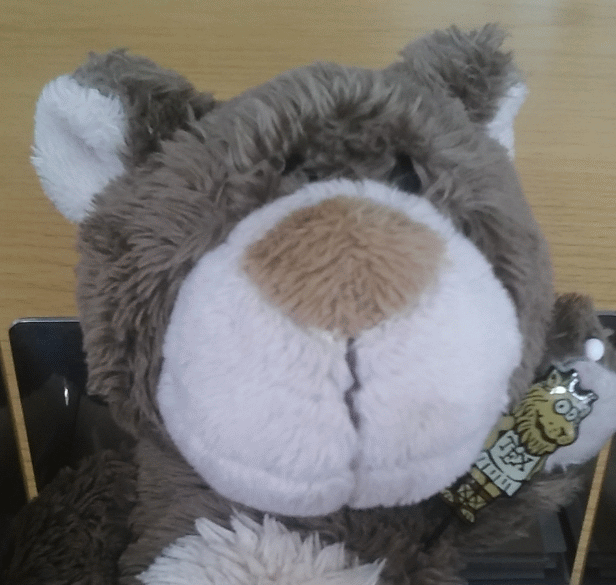
\includegraphics[width=4cm]{baer}
% \begin{description}
% \item[Ulrike]
%  Bär, your decision to create \bearwearlogo{} has come as a surprise to many. Did you expect this?
%  \item[Bär] Quite true, Ulrike. I am better known as an outdoor type
%  and the fashionistas didn't reckon with me at all.
% \item[Ulrike] So, why did you take this step?
% \item[Bär] There were quite a few reasons -- most importantly
% my deeply felt desire to bring more justice to the world.
% Look at the wonderful world of \TikZ ducks fashion, and even Marmots have come
% far in the area of refinement. Why should \TikZ bears be left behind?
% \item[Ulrike] You are also concerned with the more momentous issues of our day.
% \item[Bär] Correct! My fashion line is the first ever to have practically
% no negative influence on our environment. Manufacture and transportation
% are ecologically neutral. In fact it's the first time in the
% history of world economy that goods are produced without
% the use of raw materials.
% \item[Ulrike] You claim that \bearwearlogo{} will have a global impact.
% \item[Bär] Yes, the issue of globalization is one which has interested
%  me for a long time. \bearwearlogo{} caters for the needs of \TikZ bears all
%  over the world. There is the Longshirt Line for those who live near the poles,
%  t-shirts for those in temperate regions and even a Muscle Shirt Line for the
%  bears of Australia.
% \item[Ulrike] How about individuality?
% \item[Bär] I am particularly proud that \bearwearlogo{} enables every single
% bear to create his own personal shirt -- free of the dicatates of the modern
% Brummells. He may use my suggestions but he need not do so.
% \item[Ulrike] Will you be seen wearing your own creations?
% \item[Bär] Well Ulrike, I am afraid this is not very likely.
% I have got this most beautiful fur and I'd hate to  cover it with artifical
% patterns -- no matter how ravishing.
% \item[Ulrike] One last question: what impulse got you moving towards
% \bearwearlogo{}?
% \item[Bär] The death of Karl Lagerfeld. Someone had to fill the void.
% \end{description}
%    \begin{macrocode}
%<@@=bearwear>
%<*package>
\RequirePackage{xparse}
\ProvidesExplPackage {bearwear} {2020-01-12} {0.1}
  {A package for tikz bear fashion}
\ProcessOptions\relax
% a tikzset style to reverse the clip:
\tikzset{bearwear_reverseclip/.style={insert path={
   (current bounding box.south west) --(current bounding box.north west)
 --(current bounding box.north east) --  (current bounding box.south east)
 -- cycle} }}

%</package>
%    \end{macrocode}
% \PrintIndex
